\section{Timer-Konfiguration}
\label{sec:Timer-Konfiguration} %label erstellen für quervereise
\subsection{Aufgabenstellung}
Konfigurieren Sie Timer 1 als freilaufenden Timer. Implementieren Sie eine Software-PWM:
\begin{itemize}
	\item Erzeugen Sie ein Ausgangssignal mit einer Frequenz von 1 kHz. Messen Sie das Signal mit dem Oszilloskop.
	\item Schreiben Sie ein Programm, das ein pulsweitenmoduliertes Signal mit einer Periodendauer von 1 ms (ggfs. 10 ms) und einem einstellbaren Tastverhältnis ausgibt.
	\item Erzeugen Sie damit ein PWM-Signal, dessen Gleichanteil einen dreieckförmigen Verlauf (Frequenz ca. 1 Hz) hat.
	\item Steuern Sie mit diesem Signal eine Leuchtdiode an
\end{itemize}
Optional: Ändern Sie das Programm "Hallo World"\ so ab, dass das Blinken der LED durch zyklisches Lesen des Timer1-Registers gesteuert wird.


\subsection{Lösung}
Das Timer1 Module ist ein 16-bit Timer (Zähler der mit einer konfigurierbaren Frequenz inkrementiert wird), welcher in folgenden Betriebsarten betrieben werden kann:
\begin{itemize}
	\item Timer mode
	\item Gated Timer mode
	\item Synchronous Counter mode
	\item Asynchronous Counter mode
\end{itemize}
Die restlicher Timer (2-8) sind jeweils als 16-bit single Timer, oder als 32-bit Timer konfigurierbar. Bei den 32-bit Timern werden immer zwei Timer (2/3,4/5,6/7,8/9) zusammengefasst. Zur Konfiguration siehe Datenblatt.
\newline
Die Konfigurationsmöglichkeiten der Timer sind in Tabelle \ref{tab:timermodesettings} abgebildet, das Blockdiagramm in Abbildung \ref{image:Timer1BlockDiagramm}.\newline
\begin{table}[h]
	\centering
	\begin{tabular}{|c|c|c|c|c|}
		\hline 
		\textbf{Mode} & \textbf{TCS} & \textbf{TGATE} & \textbf{TSYNC} & \multicolumn{1}{|c|}{Clock} \\ 
		\hline 
		\multicolumn{1}{|l|}{Timer} & 0 & 0 & X&$\frac{F_{OSC}}{2}$\\ 
		\hline 
		\multicolumn{1}{|l|}{Gated Timer}  & 0 & 1 & X&$\frac{F_{OSC}}{2}$ \\ 
		\hline 
		\multicolumn{1}{|l|}{Synchronous Timer} & 1 & X & 1& T1CK pin \\ 
		\hline 
		\multicolumn{1}{|l|}{Asynchronous Timer} & 1 & X & 0& T1CK pin\\ 
		\hline 
	\end{tabular} 
	\caption{Timer Mode Settings}
	\label{tab:timermodesettings}
\end{table}
\newline Die Konfiguration von Timer1 ist in Listening \ref{lst:Timer1Conf} zu sehen. Hierbei wurde Timer1 als freilaufender Timer1 konfiguriert. Durch zyklisches Abfragen der Werte von TMR1 kann man verschiedene Zeitdifferenzen bestimmen. Die Anzahl der Inkrements pro Sekunde berechnet sich zu:
\begin{equation}\label{key}
f_{inc}=\frac{F_{OSC}}{2*Prescaler}
\end{equation}
Die Anzahl der Inkrements die man für eine bestimmte Zeitdauer benötigt berechnet sich zu:
\begin{equation}\label{key}
Inkrements=f_{inc}*t
\end{equation}
Somit benötigt man beispielsweise für 0.5ms: $0.5ms*\frac{140MHz}{2*64}≈547$ Inkrements.\newline \newline
Bevor man die Differenzen der Timerwerte ausrechnet muss man einen Typecast auf int16\_t vornehmen, durch die Interpretation als Zweierkomplemennt ist sichergestellt, das auch bei einem Überlauf des Timers die richtige Differenz berechnet wird. Ein Beispiel hierzu ist in Listening \ref{lst:Timer1OnCycle} zu sehen.
\newline Der Tastgrad ist auch variabel eingestellt, wie in Listing \ref{lst:Timer1OnCycle} zu sehen toggelt der digitale Ausgang immer zwischen HIGH und LOW, abhängig von der Anzahl an "dT"\ Increments (siehe if-Abfragen).


\begin{lstlisting}[frame=htrbl, caption={Timer1 Configuration}, label={lst:Timer1Conf}]
T1CONbits.TON = 0; // Disable Timer
//set the multiplexer to timer mode
T1CONbits.TCS = 0;   // Select internal instruction cycle clock
T1CONbits.TGATE = 0; // Disable Gated Timer mode

T1CONbits.TCKPS = 0b10; // Select 1:64Prescaler

TMR1 = 0x00; // Clear timer register
PR1 = 0xFFFF; // Load the period value

//disable interrupt
IPC0bits.T1IP = 0x00;// Set Timer 1 Interrupt Priority Level
IFS0bits.T1IF = 0; // Clear Timer 1 Interrupt Flag
IEC0bits.T1IE = 0; // Enable Timer1 interrupt 

T1CONbits.TON = 1; // Start Timer
\end{lstlisting}

\begin{lstlisting}[frame=htrbl, caption={Timer1 on Cycle}, label={lst:Timer1OnCycle}]
int16_t    _i16Timer1_1kHz_dTOn=0;
int16_t    _i16Timer1_1kHz_dTOff=0;
uint8_t    _ui8Timer1_1kHz_Port=0;

void onCycleTimer1PWM_1kHz()
{
	static uint8_t _ui8Timer1_1kHz_Mode=0;
	static int16_t _i16Timer1_1kHz_T0 = 0;
	int16_t i16_T1 = (int16_t)TMR1;
	if(_ui8Timer1_1kHz_Mode == 0)
	{
		if((i16_T1 - _i16Timer1_1kHz_T0) >= _i16Timer1_1kHz_dTOff) //_i16Timer1_1kHz_dTOff
		{
			digitalWrite(_ui8Timer1_1kHz_Port,HIGH);
			_i16Timer1_1kHz_T0 = (int16_t)TMR1;
			_ui8Timer1_1kHz_Mode=1;        
		}
	}
	else
	{
		if((i16_T1 - _i16Timer1_1kHz_T0) >= _i16Timer1_1kHz_dTOn) //_i16Timer1_1kHz_dTOn
		{
			digitalWrite(_ui8Timer1_1kHz_Port,LOW);
			_i16Timer1_1kHz_T0 = (int16_t)TMR1;
			_ui8Timer1_1kHz_Mode=0;       
		}

	}  	
}
\end{lstlisting}

\begin{figure}[h]
	\centering
	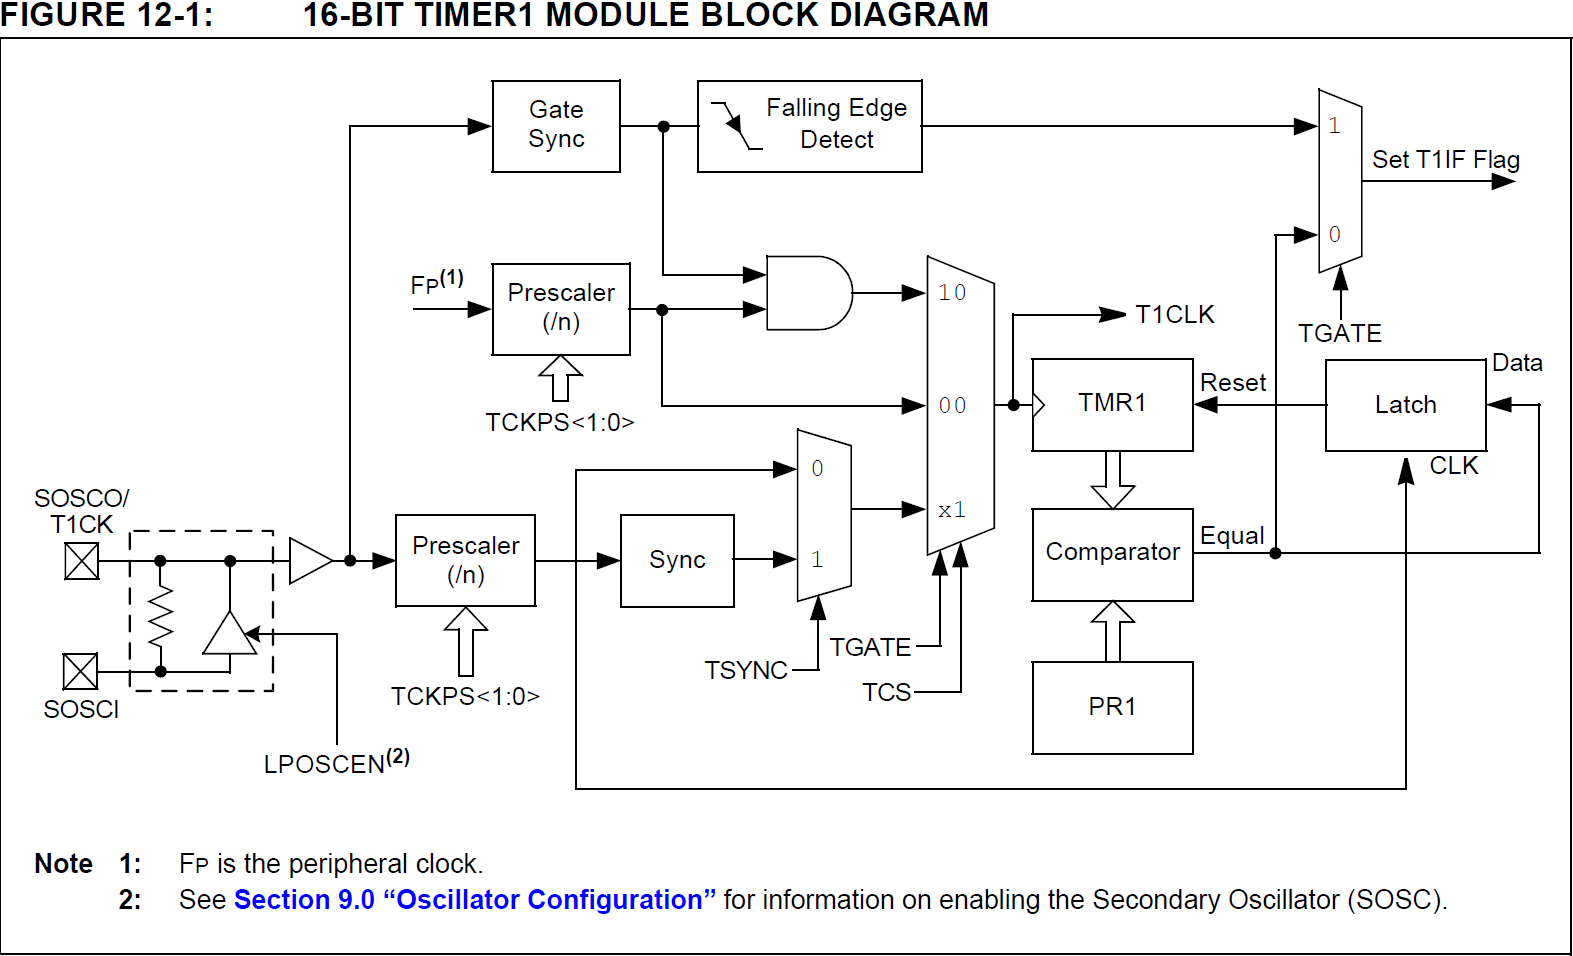
\includegraphics[width=\textwidth]{Images/timer1blockdiagramm}
	\caption[Timer1 Block Diagramm]{Timer1 Block Diagramm}
	\label{image:Timer1BlockDiagramm}
\end{figure}
